\documentclass{article}
\usepackage{graphicx} % Required for inserting images

\title{Trabajo Práctico 3 - Teoría de Juegos}
\author{Juani Elosegui}
\date{Septiembre 2024}

\begin{document}
    \maketitle

    \newpage
    
    \section*{Problema 1}
        \subsection*{Respuestas}
            \subsubsection*{Falso.}
                Jugar primero siempre tiene ventaja, pero no quiere decir que la primera jugada sea correcta siempre. Puede llegar a servirle al que juega segundo por si el que jugó primero tuvo algún error. Pero, a fin de cuentas, puede servir para patear el tablero con el reconocimiento de la marca o asegurarse un recurso escaso.

                Como el segundo jugador se puede aprovechar correctamente de la decisión del primer jugador, no siempre tiene ventaja quien juegue primero.

            \subsubsection*{Verdadero.}
                Sí es un juego válido, ya que las estrategias que puede elegir el Jugador 2 en su abanico están definidas por la decisión que tomó el Jugador 1 cuando le tocó decidir. No existe un paradigma como ese si el juego fuese simultáneo, pero sí puede pasar tranquilamente si el juego es secuencial.

    \newpage

    \section*{Problema 2}
        \subsection*{Respuestas}
            \subsubsection*{a)}
                Voy a arrancar ordenando el pago del jugador 2.
                \[P_{2} = m+a(m-(1-m))\]
                \[P_{2} = m+a(m-1+m)\]
                \[P_{2} = m+a(2m-1), a>0\]

                El juego secuencial graficado queda así:
                \begin{center}
                    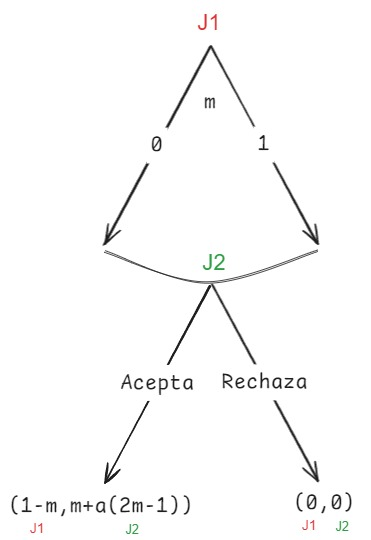
\includegraphics[width=0.4 \linewidth]{figs/fig16.jpeg}
                \end{center}

            \subsubsection*{b)}
                Uso la inducción para atrás para resolver este inciso. El Jugador 2 decidirá dependiendo de la oferta de $m$ que haga el Jugador 1.
                \\
                \\
                Sabíamos que, si el Jugador 2 acepta, recibe un total de $m+a(2m-1)$; y si rechaza, recibe un pago de $0$. El Jugador 2 aceptará el pago si es mayor o igual a cero:
                \[m+a(2m-1) \geq 0\]
                \[m \geq -a(2m-1)\]
                \[m \geq -2am+a\]
                \[m+2am \geq a\]
                \[m(1+2a) \geq a\]
                \[m \geq \frac{a}{2a+1}\]

                Es decir, aceptará siempre y cuando $m \geq \frac{a}{2a+1}$.
                \\
                \\
                El Jugador 1 sabe que el Jugador 2 acepta con la condición que dije arriba. Por eso, el Jugador 1 querrá ofrecer el menor $m$ posible con tal de que el Jugador 2 acepte, porque maximiza el pago de J1, que es $1-m$.

                Sin hacer más cuentas, el Jugador 1 ofrecerá exactamente $m = \frac{a}{2a+1}$.

            \subsubsection*{c)}
                Se puede ver que $m(a) = \frac{a}{2a+1}$ es una función estrictamente creciente. Entre mayor sea $a$, más le interesará al Jugador 2 la diferencia entre lo que recibe él y lo que recibe el Jugador 1. Por lo tanto, el Jugador 1 necesita ofrecer más para evitar que el Jugador 2 rechace la oferta.

    \newpage

    \section*{Problema 3}
        \subsection*{Respuestas}
            \subsubsection*{a)}
                \begin{center}
                    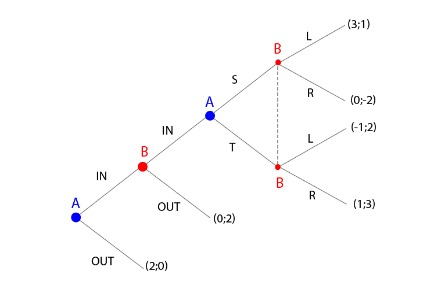
\includegraphics[width=0.5 \linewidth]{figs/fig17.jpeg}
                \end{center}

            \subsubsection*{b)}
                Tiene tres subjuegos: el conjunto de J$_{1}: S_{1} = \{IN; OUT; IN _{S}; IN_{T}\}$ y el conjunto de J$_{2}: S_{2} = \{IN_{L}; IN _{R}; OUT\}$ 

            \subsubsection*{c)}
                El Equilibrio de Nash es: $\{(S,L);(T,R)\}$
                \\
                En el subjuego 3 juegan los dos, y las mejores respuestas son las del Equilibrio de Nash de arriba. En el subjuego 2 juega el Jugador B, y la mejor respuesta es (IN, IN). En el subjuego 1 juega el Jugador A, y la mejor respuesta es (IN, OUT).
                \\
                Por lo que $ENPS:\{(IN_{S}, IN_{L});(OUT_{T}, IN_{R})\}$
    \newpage

    \section*{Problema 4}
        \subsection*{Respuestas}
            \subsubsection*{a)}
                En la primera parte de este juego secuencial, la Firma 1 elige $a$. En la segunda parte, las dos firmas compiten fijando precios en simultáneo.

                Hay dos subjuegos: el de la segunda parte y el juego completo (donde se establece $a$ y se compite en base a ello).

            \subsubsection*{b)}
                Primero, armo las funciones de utilidad de las firmas.
                \[U_{1}(p_{1}, p_{2}) = p_{1} \cdot q_{1}\]
                \[U_{1}(p_{1}, p_{2}) = p_{1} \cdot (10a-2p_{1}+p2)\]
                \[U_{2}(p_{1}, p_{2}) = p_{2} \cdot q_{2}\]
                \[U_{2}(p_{1}, p_{2}) = p_{2} \cdot (10a-2p_{2}+p_{1})\]

                La idea ahora es encontrar las condiciones de primer orden, para eso hay que derivar las funciones de utilidad de cada firma con cada precio.
                \[\frac{\partial U_{1}}{\partial p_{1}} = 0\]
                \[\frac{\partial}{\partial p_{1}}(10ap_{1}-2p^{2}_{1}+p_{1}p_{2}) = 0\]
                \[10a-4p_{1}+p_{2} = 0\]
                \[p_{1} = \frac{10a+p_{2}}{4}\]

                Esta será la mejor respuesta de la Firma 1: $p_{1} = \frac{10a+p_{2}}{4}$. Ahora, para buscar la mejor respuesta de la Firma 2, hago lo mismo:
                \[\frac{\partial U_{2}}{\partial p_{2}} = 0\]
                \[\frac{\partial}{\partial p_{2}}(10ap_{2}-2p^{2}_{2}+p_{1}p_{2}) = 0\]
                \[10a-4p_{2}+p_{1} = 0\]
                \[p_{2} = \frac{10+p_{1}}{4}\]

                Si reemplazamos $p_{1}$ en $p_{2}$ o viceversa, llegaríamos a que los precios de equilibrio son: $p_{1}^{*} = p_{2}^{*} = \frac{10a}{3}$.
                
            \subsubsection*{c)}
                Para encontrar los Equilibrios de Nash perfectos en subjuegos primero tengo que partir del caso en el cual la Firma 1 elige $a$ para maximizar sus ganancias, recordando que $C(a) = a^3$. Planteamos primero la utilidad de la Firma 1 en el juego (completo) y reemplazamos los precios por los que encontramos en el equilibrio:
                \[U_{1} = p_{1}^{*} \cdot q_{1} - a^{3}\]
                \[U_{1} = (\frac{10a}{3}) \cdot (10a-2\frac{10a}{3}+\frac{10a}{3})-a^{3}\]

                Cálculos más, cálculos menos, llegué a que la utilidad de la Firma 1 es:
                \[U_{1} = \frac{200a^{2}}{9}-a^{3}\]

                Para encontrar el valor adecuado de $a$, hay que hacer la derivada parcial de $U_{1}$ con respecto a $a$ e igualarlo a cero:
                \[\frac{\partial U_{1}}{\partial a} = \frac{400}{9}a-3a^{2}\]
                \[\frac{\partial U_{1}}{\partial a} = 0\]
                \[\frac{400}{9}a-3a^{2} = 0\]
                \[a(\frac{400}{9}-3a) = 0\]
                \[a_{1} = 0 \vee a_{2} = \frac{400}{27}\]
        
\end{document}
